\documentclass[border=10pt]{standalone}
\usepackage{graphicx}
\usepackage{tikz}
\usepackage{xcolor}
\usetikzlibrary{arrows.meta, positioning, fit, backgrounds}
\definecolor{academicblue}{RGB}{30,64,105}
\definecolor{accent}{RGB}{180,120,40}
\definecolor{muted}{RGB}{100,116,139}
\begin{document}
\resizebox{8.4cm}{!}{%
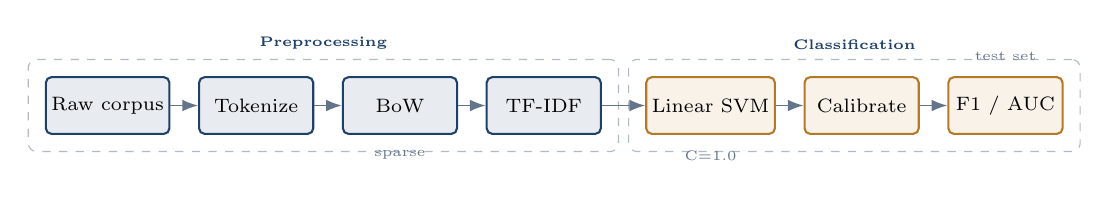
\begin{tikzpicture}[
  font=\scriptsize,
  box/.style={rectangle, rounded corners=2pt, draw=#1, line width=0.75pt,
    fill=#1!10, minimum width=1.45cm, minimum height=0.72cm, align=center, inner sep=2pt},
  group/.style={draw=muted!50, dashed, rounded corners=3pt, inner sep=6pt},
  arr/.style={-{Latex[length=2mm]}, draw=muted, line width=0.55pt},
  lbl/.style={font=\tiny, text=muted}
]
\node[box=academicblue] (raw) {Raw corpus};
\node[box=academicblue, right=0.35cm of raw] (tok) {Tokenize};
\node[box=academicblue, right=0.35cm of tok] (bow) {BoW};
\node[box=academicblue, right=0.35cm of bow] (tfidf) {TF-IDF};
\node[box=accent, right=0.55cm of tfidf] (svm) {Linear SVM};
\node[box=accent, right=0.35cm of svm] (cal) {Calibrate};
\node[box=accent, right=0.35cm of cal] (met) {F1 / AUC};
\begin{scope}[on background layer]
  \node[group, fit=(raw)(tok)(bow)(tfidf), label={[font=\tiny\bfseries, text=academicblue]above:Preprocessing}] {};
  \node[group, fit=(svm)(cal)(met), label={[font=\tiny\bfseries, text=academicblue]above:Classification}] {};
\end{scope}
\foreach \x/\y in {raw/tok,tok/bow,bow/tfidf,tfidf/svm,svm/cal,cal/met}
  \draw[arr] (\x) -- (\y);
\node[lbl, below=0.08cm of bow] {sparse};
\node[lbl, below=0.08cm of svm] {C=1.0};
\node[lbl, above=0.08cm of met] {test set};
\end{tikzpicture}%
}
\end{document}
